\newcommand{\dataname}{Data1.txt}
\newcommand{\datadate}{01/01/2013 }
\newcommand{\datamean}{0}
\newcommand{\datavar}{0}
\newcommand{\datamax}{0}
\newcommand{\datamin}{0}
\newcommand{\datasum}{0}
\newcommand{\datahouraverage}{0}






\documentclass{article}
\usepackage{graphicx}
\begin{document}
\title{AutoReport of \dataname}
\author{Jorge Luis Mayorga}
\date{\datadate}
\maketitle
\line(1,0){300} 

\section{Resumen del Dia}
Buenas noches a todos, en la presente se adjuntan los balances del dia \datadate           cuyos resultados estadisticos arrojan que :
\begin{itemize}
\item La media es de \datamean
\item La varianza es de \datavar
\item El dato maximo es de \datamax
\item El dato minimo es de \datamin
\item El acumulado en el dia es \datasum
\item El promedio por hora es de \datahouraverage
\end{itemize}

\section{Grafica}

\begin{figure}
  \centering
    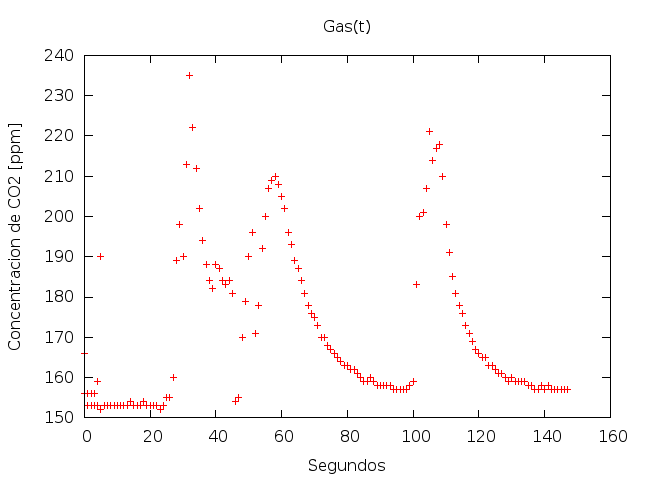
\includegraphics[width=1\columnwidth]{Plot_data.png}
  \caption{Grafica de Dia \datadate}
  \label{fig:plot}
\end{figure}



\end{document}